\documentclass[Main]{subfiles}
\begin{document}

\chapter{Elicitation Process}\label{cha:Elicitation}

\begin{wrapfigure}{r}{0.5\textwidth}
\begin{center}
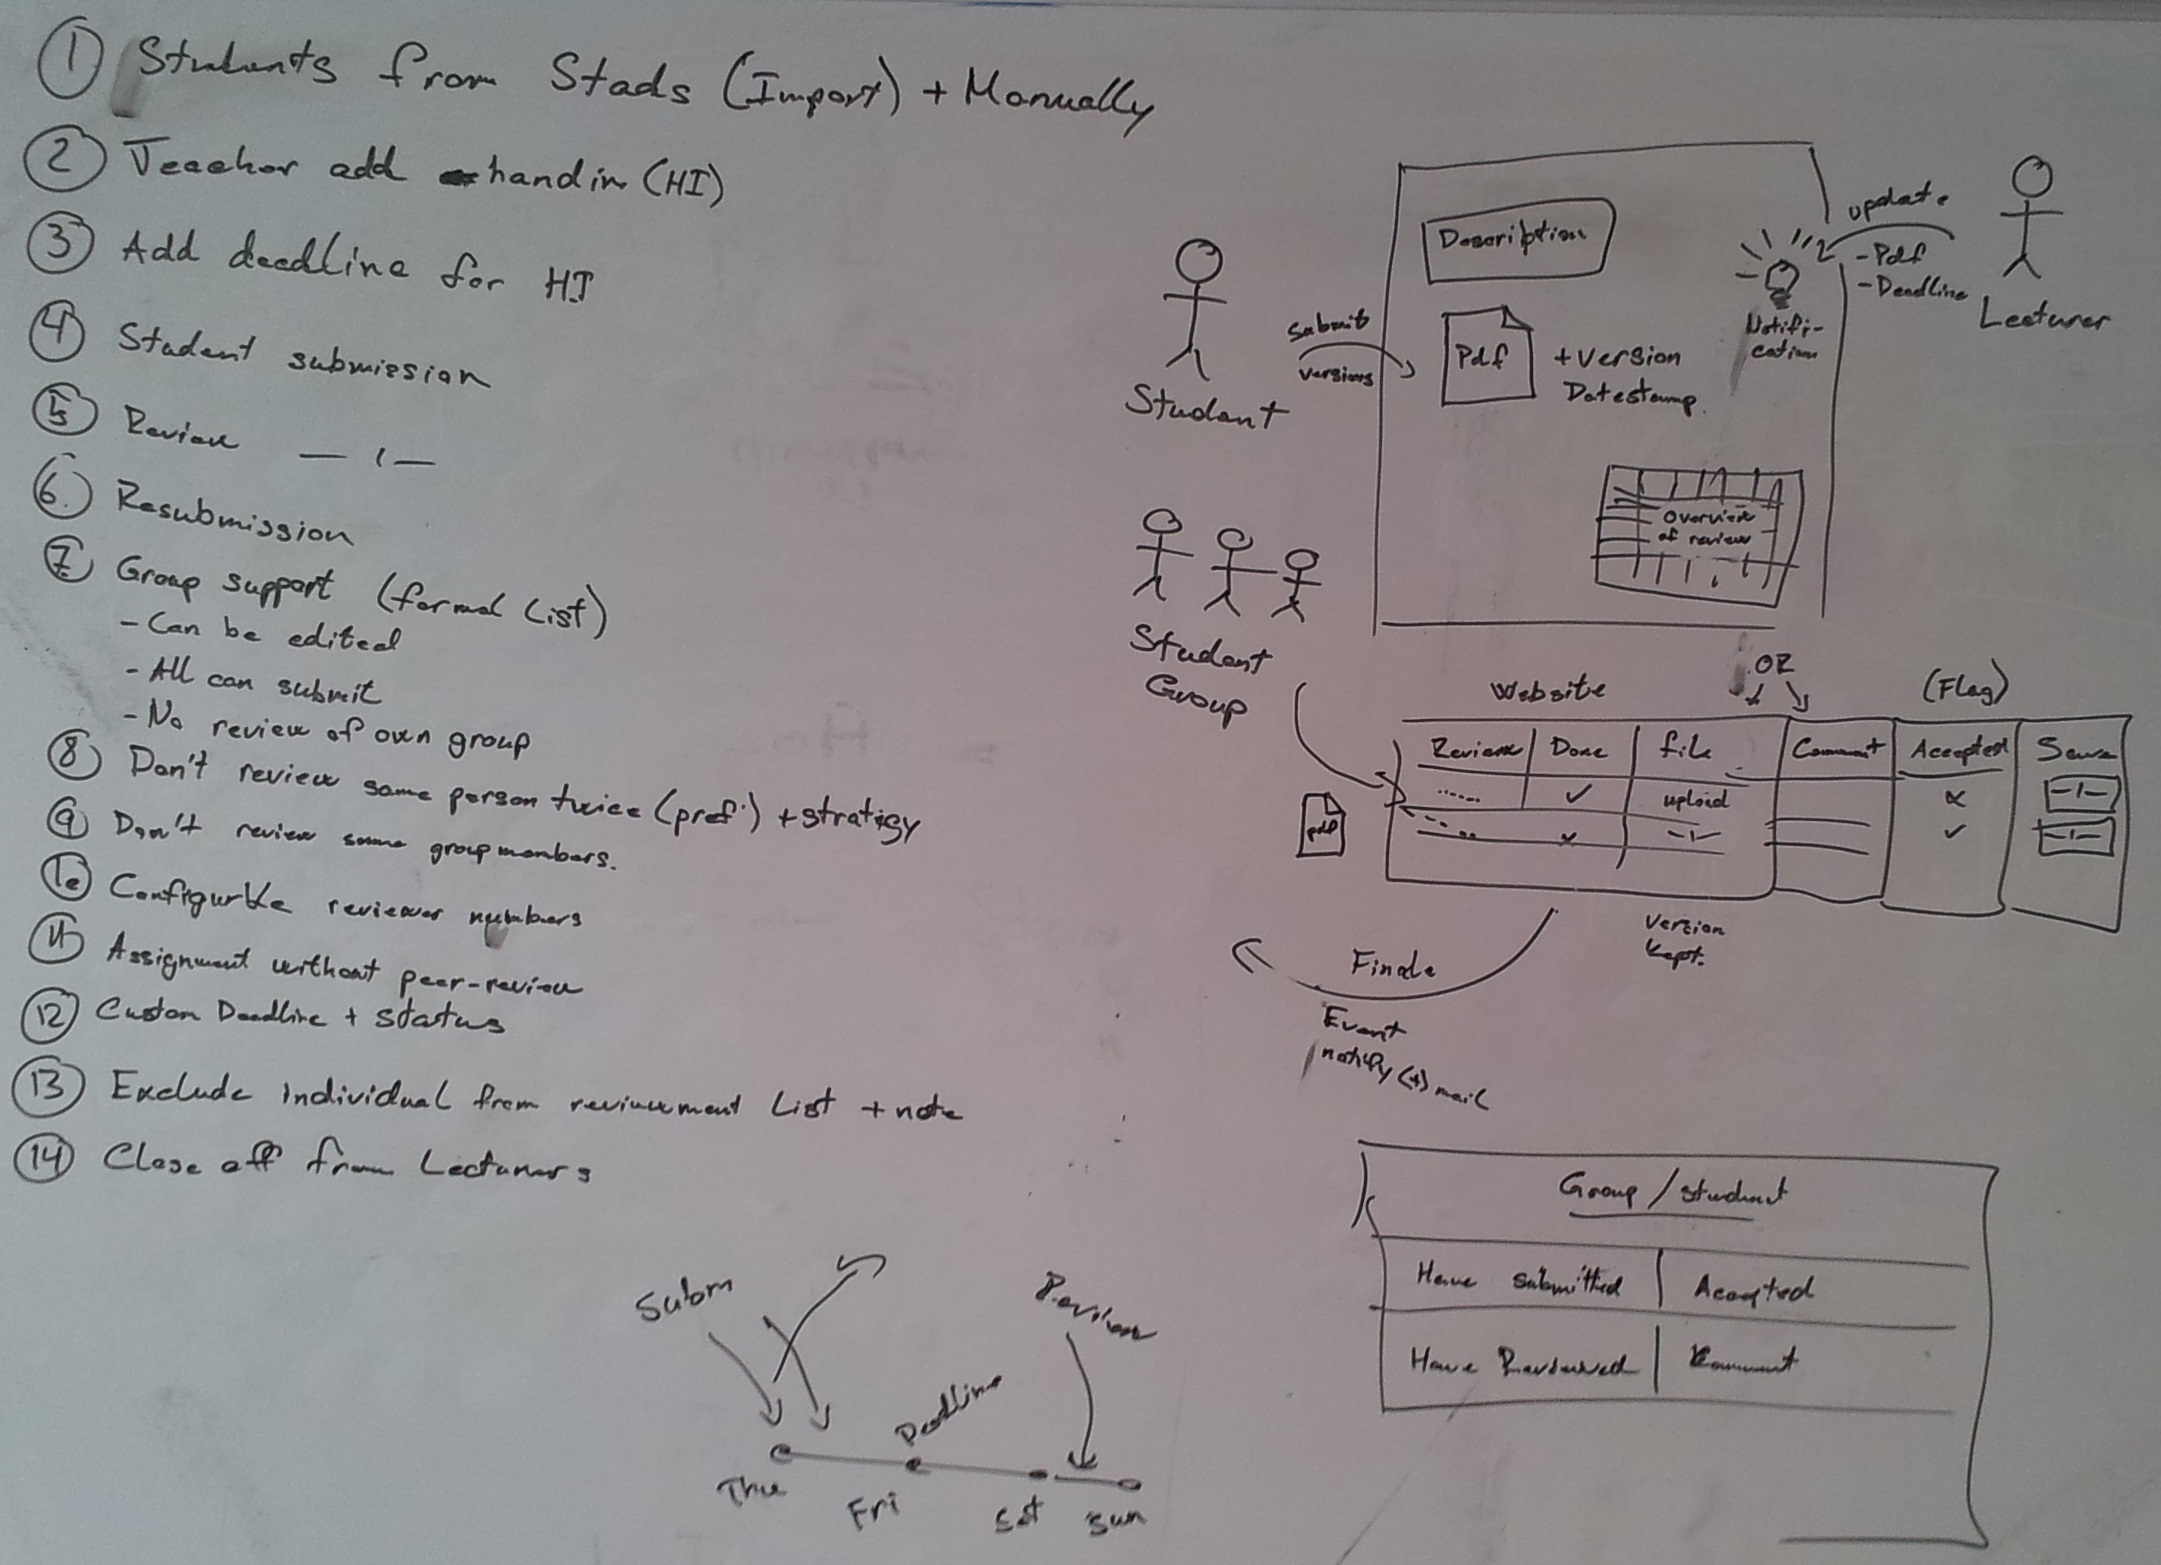
\includegraphics[width=0.48\textwidth]{IMG_20140221_131547.jpg}
\end{center}
\caption{Whiteboard notes created during user interview.}
\label{fig:UserInterviewNotes}
\end{wrapfigure}

%In this chapter, "we" refers to the group carrying out the elicitation process.
This chapter describes the elicitation process carried out to create this requirement specification. \\



Used:
\begin{itemize}
\item Observation - Work process was observed as a user by participating in the course
\item User interviews - 2 with Joey(+notes)
\item Stakeholder analysis(implicit) - Finding the goal of the customer helped understand the system.
\end{itemize}


Not used:
\begin{itemize}
\item Questionnaires - Was outside the scope of this project.
\item Brainstorm - New ideas was not needed.
\item Domain workshop - Not needed. The system was well-understood.
\item Focus group
\end{itemize}




\end{document}